% -*- TeX:de -*-
\NeedsTeXFormat{LaTeX2e}
\documentclass[12pt,a4paper,titlepage]{article}

%\usepackage[german]{babel} % german text
\usepackage[DIV12]{typearea} % size of printable area
\usepackage[T1]{fontenc} % font encoding
\usepackage[utf8]{inputenc} % probably on Linux

\usepackage{graphicx} % to include images
\usepackage{subfigure} % for creating subfigures
\usepackage{amsmath} % a bunch of symbols
\usepackage{amssymb} % even more symbols
\usepackage{booktabs} % pretty tables
\usepackage{csquotes}

% a floating environment for circuits
\usepackage{float}
\usepackage{caption}

\usepackage[european]{circuitikz}
\ctikzset{voltage/distance from line=.25}% pos. between 0 and 1

\newfloat{circuit}{tbph}{circuits}
\floatname{circuit}{Schaltplan}

% a floating environment for diagrams
\newfloat{diagram}{tbph}{diagrams}
\floatname{diagram}{Diagramm}

\renewcommand{\familydefault}{\sfdefault} % activate to use sans-serif font as default

\sloppy % friendly typesetting

\usepackage{eurosym}
%\usepackage{makeidx}
\usepackage{amsfonts}
\usepackage{mparhack}
\usepackage{array}
\usepackage{tabularx}
\usepackage{minitoc}
\usepackage[colorlinks=true]{hyperref}
\usepackage{epstopdf}
\usepackage{setspace}
\usepackage{csquotes}

\usepackage{pgfplots}
\usetikzlibrary{automata,arrows,chains,shapes.misc,scopes,petri}

\usepackage{csvsimple}
\usepackage{siunitx,array,booktabs}
\usepackage{longtable}
\usepackage[pass]{geometry}

\begin{document}

\begin{titlepage}

\begin{figure*}[h!]
  \includegraphics[width=8cm]{TULogo_CMYK}
\end{figure*}

\begin{center}
\vspace*{1.3cm}
{\Huge Elektrotechnische Grundlagen der Informatik\\(LU 182.692)\\}
\vspace{1.7cm}
{\LARGE Protokoll der 3. Laborübung: \enquote{Operationsverstärker}\\}
{\LARGE b) Messungen\\}
\vspace{1.5cm}

% fill in group number and date of lab here
% CHANGE ME!
{\Large Gruppennr.: 10 \hspace{1cm} Datum der Laborübung: 01.06.2017}

% fill in IDs and names here
% CHANGE ME!
\begin{table}[h!]
\centering
\begin{tabular}{|p{3.5cm}|p{3.5cm}|p{6.5cm}|}
\hline \textbf{Matr. Nr.} & \textbf{Kennzahl} & \textbf{Name} \\
\hline
1609418 & 033 535 & GEISELBRECHTINGER Max \\
\hline
1625753 & 033 535 & HAAR Martin \\
\hline
& & \\
\hline
\end{tabular}
\end{table}

\end{center}
\vspace{1.0cm}

\begin{table}[h!]
\begin{tabular}{|l|l|}
\hline \textbf{Kontrolle} & \checkmark \\
\hline Nichtinvertierender OPV & \\
\hline OPV und Grenzfrequenz & \\
\hline Invertierender OPV & \\
\hline Integrierer & \\
\hline Schmitt-Trigger & \\
\hline
\end{tabular}
\end{table}

\end{titlepage}
\setcounter{page}{2}

%only sections in tableofcontents, no subsections
\setcounter{tocdepth}{1}
%sets tableofcontents color black
\hypersetup{linkcolor=black}

% start of actual lab protocol
% CHANGE ME!
\tableofcontents
% !TEX root = deckblatt3b.tex

\section{Nicht-Invertierender Verst\"arker}

In dieser Aufgabe sollte eine nichtinvertierende Operationsverstärkerschaltung aufgebaut und anschließend das Verhalten im
Gleich- und Wechselspannungsbetrieb ermittelt werden. Die Verstärkung war mit einem Faktor von 40-60 zu wählen.\\

\subsection{Schaltung}
\begin{figure}[H]
  \begin{center}
    %\tikzset{component/.style={draw,thick,circle,fill=white,minimum size =0.75cm,inner sep=0pt}}
    \resizebox{0.7\linewidth}{!}{
      \begin{circuitikz}
        \draw (0,0)
        (3,4) node[op amp,yscale=-1] (opamp) {}
        (3,4.5) to[short] (3,5) node[vcc] {$V_{CC}$}
        (3,3.5) to[short] (3,3) node[vss] {$V_{SS}$}
        (opamp.+) to[short] (0,4.5)
        (opamp.-) to[short] (1.5,3.5) to[short] (1.5,1.5) to[short] (4.5,1.5){}
        (4.5,4) to[R={$R_2$}] (4.5,1.5) to[R={$R_1$}] (4.5,-0.5) node[ground] (ground) {}
        (opamp.out) to[short] (8,4)
        (8,-0.5) node[ground] (ground) {}
        (0,-0.5) node[ground] (ground) {}
        ;
        \draw (0,4.2) to[short] (0,0.2) node[vee] {};
        \draw (-0.5,2.2) node[] {$U_e$};
        \draw (8,3.7) to[short] (8,0.2) node[vee] {};
        \draw (8.5,1.7) node[] {$U_a$};

      \end{circuitikz}
    }
    \caption{nicht inververtierender OPV}
  \end{center}
\end{figure}
\noindent
Der Operationsverstärker wurde mit $\pm15V$ versorgt und die Widerstände wurden wie folgt gewählt.\\
\begin{align*}
 R_1 &= 1k\Omega, R_2 = 47k\Omega\\
 -\frac{U_a}{U_e} &= \frac{R_1 + R_2}{R_1}\\
 U_a &= -U_e(1 + \frac{R_2}{R_1})\\
 U_a &= -48*U_e\\
\end{align*}

\subsection{Gleichspannungsverhalten}

Um das Verhalten im Gleichspannungsbetrieb zu ermitteln wurde der OPV zuerst mit einer Eingangsspannung von $100mV$ und anschließend
mit $300mV$ beaufschlagt.\\

\begin{table}[H]
\begin{minipage}{.5\textwidth}
\begin{figure}[H]
\centering
 \begin{tabular}{c|c}
  $U_e$ & $99,7mV$ \\ \hline
  $U_a$ & $4,8V$ \\ \hline
  $U_{R1}$ & $100mV$ \\ \hline
  $U_{R2}$ & $4,73V$ \\ \hline
  $U_d$ & $-0,5mV$ \\ \hline
  $I_{R1}$ & $0,096mA$ \\ \hline
  $I_{R2}$ & $0,101mA$ \\ \hline
  $I_+$ & $0mA$ \\ \hline
  $I_-$ & $0mA$ \\
 \end{tabular}
  \caption{Messwerte $0,1V$ DC}
\end{figure}
\end{minipage}
\begin{minipage}{.5\textwidth}
\begin{figure}[H]
  \centering
 \begin{tabular}{c|c}
  $U_e$ & $299mV$ \\ \hline
  $U_a$ & $14,21V$ \\ \hline
  $U_{R1}$ & $295mV$ \\ \hline
  $U_{R2}$ & $13,91V$ \\ \hline
  $U_d$ & $4,4mV$ \\ \hline
  $I_{R1}$ & $0,298mA$ \\ \hline
  $I_{R2}$ & $0,298mA$ \\ \hline
  $I_+$ & $0mA$ \\ \hline
  $I_-$ & $0mA$ \\
 \end{tabular}
 \caption{Messwerte $0,3V$ DC}
\end{figure}
\end{minipage}
\end{table}
\noindent
In den Messwerten kann man die lineare 48-fache Verstärkung der Eigangsspannung erkennen. Betrachtet man einen
idealen Operationsverstärker so sollten die Ströme an den Eingängen gleich null und die Spannung am Widerstand $R_1$
gleich der Eingangsspannung sein. Diese Annahme stimmt auch gut mit den Messwerten überein. Auch die Ströme an den
beiden Widerständen sind nahezu gleich groß, dies ist erforderlich um die Spannungsteilerregel in der Übertragungsfunktion
verwenden zu können.\\

\subsection{Wechselspannungsverhalten}

Zum protokollieren des Wechselspannungsverhalten sollte ein Rechtecksignal an den OPV angelegt und dessen Frequenz variiert
werden.\\

\begin{figure}[H]
 \begin{center}
  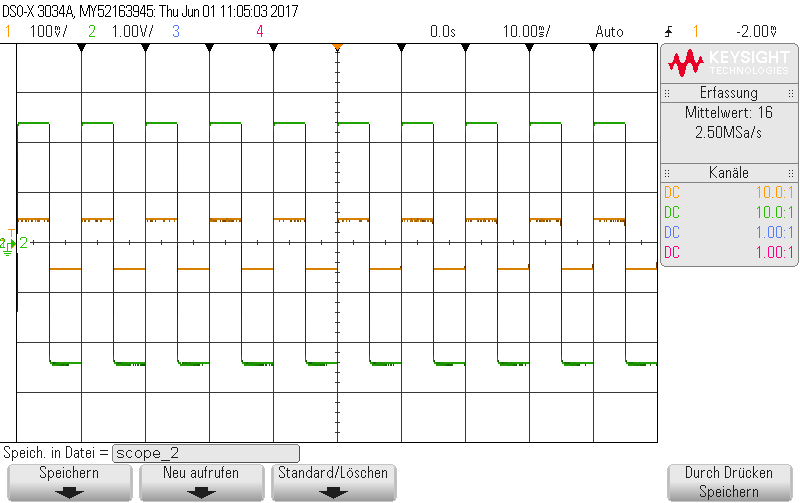
\includegraphics[height=6cm,width=12cm]{OsziBilder/nichtInvVer_100Hz}
 \end{center}
 \caption{Rechteckspannung $0,1V_{pp}$, $100Hz$ ($U_e$ orange, $U_a$ grün)}
\end{figure}

\begin{figure}[H]
 \begin{center}
  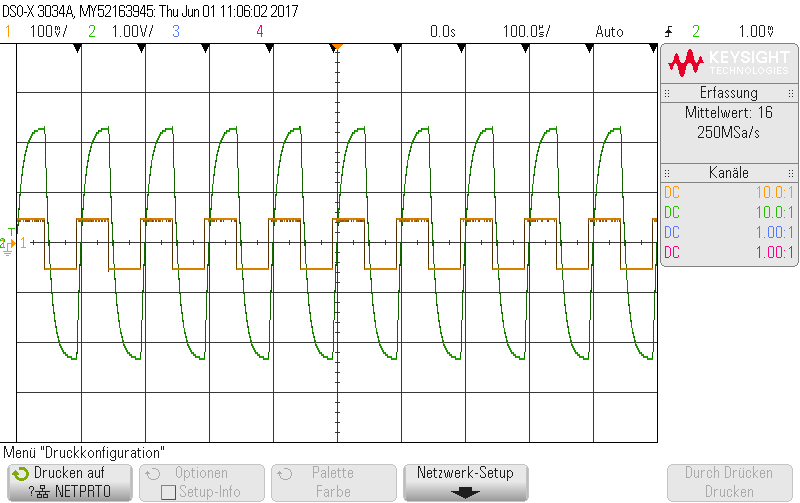
\includegraphics[height=6cm,width=12cm]{OsziBilder/nichtInvVer_10kHz}
 \end{center}
 \caption{Rechteckspannung $0,1V_{pp}$, $10kHz$ ($U_e$ orange, $U_a$ grün)}
\end{figure}
\noindent
Das $100Hz$ Signal zeigt eine schöne $1:48$ Übertragung. Bei $10kHz$ jedoch
wurde die Grenzfrequenz der Operationsverstärkerschaltung überschritten und das bauteilbedingte Tiefpassverhalten wirkt sich
auf die Ausgangsspannung aus. Daher wird das Signal nicht mehr korrekten Verhältnis verstärkt und verschliffen übertragen.\\

% !TEX root = deckblatt3b.tex

\section{Invertierender Verst\"arker}
\subsection{Aufgabenstellung}
Es soll ein invertierender OPV aufgebaut werden und desen Funktion durch Stom- und Spannungsmessung gepr\"uft werden. Anschlie\ss{}end soll das Frequnezverhalten des OPVs mithilfe von Bodediagrammen festgehalten werden.

\subsection{Schaltung}

\begin{figure}[H]
  \begin{center}
    %\tikzset{component/.style={draw,thick,circle,fill=white,minimum size =0.75cm,inner sep=0pt}}
    \begin{circuitikz}
      \draw (0,0)
      (0,4) to[R=$R_2$] (opamp)
      node[op amp,yscale=-1] (opamp) {}
      (opamp.+) to[short] (4,4)

      (4,4) node[op amp,yscale=-1] (opamp) {}
      ;

    \end{circuitikz}
    \caption{nicht inververtierender OPV}
  \end{center}
\end{figure}
\noindent
Da es sich bei dieser Schlatung um einen invertierenden Verst\"arker handelt, wird die Eingangsspannung an den invertierenden Eingang des OPV geschaltet.
Der Ausgang wird ebenfalls auf den invertierenden Eingang gegengekoppelt, um eine brauchbare Verst\"arkung einstellen zu k\"onnen. Ein Idealer OPV ohne Gegenkopplung w\"urde die Differenzspannung zwischen invertierenden und nicht-invertierenden Eingang $\infty$ verst\"arken. Die Verst\"arkung wird mit den beiden Widerst\"anden $R_1$
und $R_2$ eingestellt. Die beiden Spannungsquellen $V_2$ und $V_3$ stellen die symmetrische Versorgungsspannung von $-15V$ bis $+15V$ dar.\\ \\
$\frac{U_e}{U_a}=-\frac{R_1}{R_2} \Rightarrow U_a=-U_e*\frac{R_2}{R_1} \Rightarrow V=-\frac{R_2}{R_1}$ \\ \\
Da sich die Verst\"arkung $V$ laut Angabe zwischen $-40$ und $-60$ befinden soll wurden f\"ur die Widerst\"ande folgende Werte gew\"ahlt: \\ \\
$R_1=82k\Omega$ \\
$R_2=1,5k\Omega$ \\
$V=-\frac{82k \Omega}{1,5k\Omega}=-54,7$

\subsection{Strom- und Spannungsmessung}
\begin{table}[H]
\begin{minipage}{.5\textwidth}
\begin{figure}[H]
\centering
 \begin{tabular}{c|c}
  $U_e$ & $96,4mV$ \\ \hline
  $U_a$ & $-5,2V$ \\ \hline
  $U_{R1}$ & $95,6mV$ \\ \hline
  $U_{R2}$ & $-5,15V$ \\ \hline
  $U_d$ & $-0,4mV$ \\ \hline
  $I_{R1}$ & $63\mu A$ \\ \hline
  $I_{R2}$ & $63\mu A$ \\ \hline
  $I_+$ & $0mA$ \\ \hline
  $I_-$ & $0mA$ \\
 \end{tabular}
  \caption{Messwerte $0,1V$ DC}
\end{figure}
\end{minipage}
\begin{minipage}{.5\textwidth}
\begin{figure}[H]
  \centering
 \begin{tabular}{c|c}
  $U_e$ & $309,1mV$ \\ \hline
  $U_a$ & $-13,6V$ \\ \hline
  $U_{R1}$ & $265,2mV$ \\ \hline
  $U_{R2}$ & $-14,39V$ \\ \hline
  $U_d$ & $-575mV$ \\ \hline
  $I_{R1}$ & $169\mu A$ \\ \hline
  $I_{R2}$ & $169\mu A$ \\ \hline
  $I_+$ & $0mA$ \\ \hline
  $I_-$ & $0mA$ \\
 \end{tabular}
 \caption{Messwerte $0,3V$ DC}
\end{figure}
\end{minipage}
\end{table}
\noindent
Die Strom- und Spannungsmessungen wruden mit zwei verschiedenen Eingangsspannungen durchgef\"uhrt, einmal mit $100mV$ Gleichspannung und einmal mit $300mV$ Gleichspannung. Die Messungen passen sehr gut mit den Simulationsergebnissen \"uberein. \\
Man kann in den Messungen die Verst\"arkung lt. Messung betr\"agt $V=\frac{-5.2}{0.0964}=-53,9$ Dieser Wert passt mit der errechneten Verst\"arkung von $V=-54,7$ sehr gut \"uberein. Die Str\"ome welche an den Eing\"angen in den OPV flie\ss{} waren zu klein um sie mit dem Ampermeter messen zu k\"onnen, dies stimmt mit der Theorie sehr gut \"uberein da bei einem idealen OPV auf Grund des unendlich großen Eingangswiderstandes kein Strom hineinflie\ss{}en kann. Der Srom durch die Beiden Widerst\"ande ist ebenfalls wie erwartet der gleiche.

\subsection{Messungen im Zeitbereich}
\begin{figure}[H]
 \begin{center}
  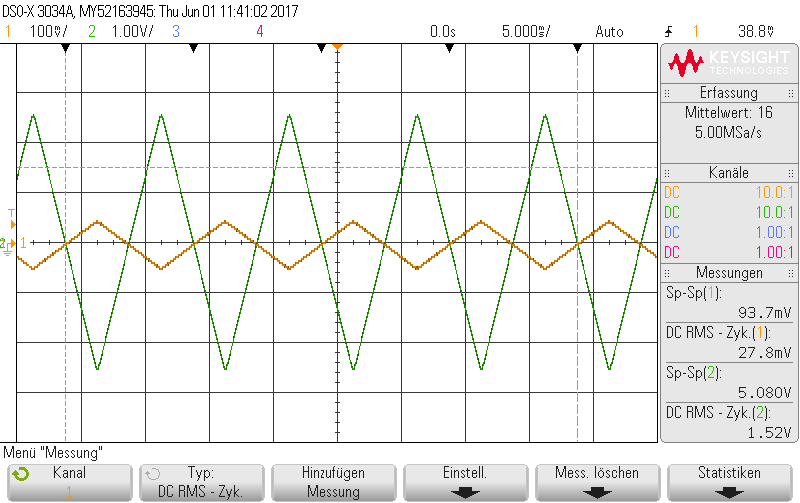
\includegraphics[height=6cm,width=12cm]{OsziBilder/InvVer_100Hz}
 \end{center}
 \caption{Dreieckspannung $0,1V_{pp}$, $100Hz$ ($U_e$ orange, $U_a$ grün)}
\end{figure}

\begin{figure}[H]
 \begin{center}
  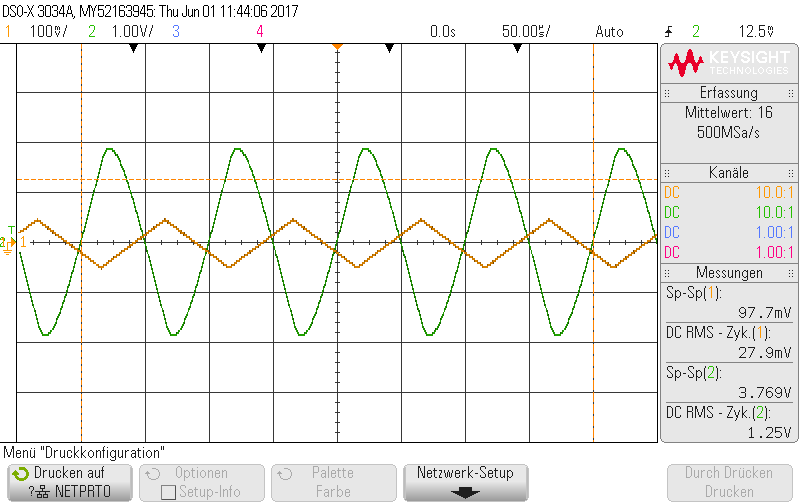
\includegraphics[height=6cm,width=12cm]{OsziBilder/InvVer_10kHz}
 \end{center}
 \caption{Dreieckspannung $0,1V_{pp}$, $10kHz$ ($U_e$ orange, $U_a$ grün)}
\end{figure}
\noindent
Das $100Hz$ Signal zeigt eine schöne invertierte $1:48$ Übertragung. Bei $10kHz$ jedoch
wurde die Grenzfrequenz der Operationsverstärkerschaltung überschritten und das bauteilbedingte
Tiefpassverhalten wirkt sich aus. So wird das Signal nicht mehr korrekt Verstärkt und verschliffen übertragen.\\
\newpage


\subsection{Bodediagramm}
Es sollten zwei Bodediagramme aufgenommen werden, f\"ur beide wurde eine Sinusspannung mit $100mVpp$ als Eingnagssingal gew\"ahlt. Bei der zweiten Messung wurde die Verst\"arkung um den Fatkor 10 veringert, dies wurde durch eine Verringerung des Widerstandes $R_2$ von $82k\Omega$ auf $8,2k\Omega$ bewerkstelligt.

\begin{figure}[H]
  \centering
  \begin{tikzpicture}
    \begin{axis}[width=15cm, height=7cm, xmode=log, xmin=10, xmax=1e6, xlabel={Frequenz [Hz]}, ylabel={Amplitude [dB]},y tick label style={grid=major}]
      \addplot table[x=Frequenz, y=dB, col sep=comma] {./csv_files/invVer_bigAmpl.csv};
      %\node[label={260:{$f_g$}},circle,fill=black,inner sep=3pt] at (axis cs:15580,12) {};
    \end{axis}
  \end{tikzpicture}
  \caption{invertierender Verst\"arker, $V=-54,7$, Amplitudengang}
\end{figure}
\begin{figure}[H]
  \centering
  \begin{tikzpicture}
    \begin{axis}[width=15cm, height=7cm, xmode=log, xmin=10, xmax=1e6, xlabel={Frequenz [Hz]}, ylabel={Phase [$^\circ$]},y tick label style={grid=major}]
      \addplot table[x=Frequenz, y=Phi, col sep=comma] {./csv_files/invVer_bigAmpl.csv};
      %\node[label={260:{$f_g$}},circle,fill=black,inner sep=3pt] at (axis cs:15580,12) {};
    \end{axis}
  \end{tikzpicture}
  \caption{invertierender Verst\"arker, $V=-54,7$, Phasengang}
\end{figure}
\noindent
In diesem Bodediagramm ist sehr gut die Transitfrequnezn von $1MHz$ zu erkennen. Da sich ein realer OPV intern wie ein Tiefpassfilter verh\"alt nimmt die Verst\"arkung von der Grenzfrequnez bis zur Transitfrequnez mit $-20dB/DEK$ ab. Eine Verst\"arkung von $-54,7$ entspricht $34,76dB$ d.h. die D\"ampfung wird bei dieser Beschaltung erst ab $10kHz$ bemerkbar.

\begin{figure}[H]
  \centering
  \begin{tikzpicture}
    \begin{axis}[width=15cm, height=7cm, xmode=log, xmin=10, xmax=1e6, xlabel={Frequenz [Hz]}, ylabel={Amplitude [dB]},y tick label style={grid=major}]
      \addplot table[x=Frequenz, y=dB, col sep=comma] {./csv_files/invVer_smlAmpl.csv};
      %\node[label={260:{$f_g$}},circle,fill=black,inner sep=3pt] at (axis cs:15580,12) {};
    \end{axis}
  \end{tikzpicture}
  \caption{invertierender Verst\"arker, $V=-5,47$, Amplitudengang}
\end{figure}
\begin{figure}[H]
  \centering
  \begin{tikzpicture}
    \begin{axis}[width=15cm, height=7cm, xmode=log, xmin=10, xmax=1e6, xlabel={Frequenz [Hz]}, ylabel={Phase [$^\circ$]},y tick label style={grid=major}]
      \addplot table[x=Frequenz, y=Phi, col sep=comma] {./csv_files/invVer_smlAmpl.csv};
      %\node[label={260:{$f_g$}},circle,fill=black,inner sep=3pt] at (axis cs:15580,12) {};
    \end{axis}
  \end{tikzpicture}
  \caption{invertierender Verst\"arker, $V=-5,47$, Phasengang}
\end{figure}
\noindent
F\"ur diese Messung wurde wie oben bereits beschrieben die Verst\"arkung um den Faktor 10 verringert. Da nun de Ferst\"arkung um den Faktor 10 kleiner ist macht sich auch die D\"ampfung des OPVs erst eine Dekade sp\"ater bemerkbar, ab dann f\"alls sie jedoch genauso mit -20dB/Dek ab.
\newpage

% !TEX root = deckblatt3b.tex

\section{Integrierer}
\subsection{Aufgabenstellung}
Es soll ein Integrierer aufgebaut und dessen Funktion überpr\"uft werden. Anschlie\ss{}end soll die Funktion des Integrierers erl\"autert werden.
\subsection{Schaltung}
\begin{figure}[H]
  \begin{center}
    %\tikzset{component/.style={draw,thick,circle,fill=white,minimum size =0.75cm,inner sep=0pt}}
      \begin{circuitikz}
      \draw
      (-2,2) node[ground] (ground) {}
      (3,4) node[op amp] (opamp) {}
      (3,4.5) to[short] (3,5) node[vcc] {$V_{CC}$}
      (3,3.5) to[short] (3,3) node[vss] {$V_{SS}$}
      (opamp.-) to[R={$R$}{$=2,2k$},v=$U_R$] (-2,4.5)
      (opamp.+) to[short] (1.5,3.5) to[short] (1.5,2) node[ground] (ground) {}

      (1.5,4.5) to[short] (1.5,7.5) to[C={$C$}{$=1\mu$},v=$U_C$] (4.5,7.5) to[short] (4.5,4)
      (1.5,7.5) to[short] (1.5,9) to[R=$220k$] (4.5,9) to[short] (4.5,7.5)
      (opamp.out) to[short] (6,4)
      (6,2) node[ground] (ground) {}
      ;
      \draw (-2,4.2) to[short] (-2,2.7) node[vee] {};
      \draw (-1.5,3) node[] {$U_e$};
      \draw (6,3.7) to[short] (6,2.7) node[vee] {};
      \draw (6.5,3) node[] {$U_a$};
      \draw (4.1,3.5) node[] {LM741};
      \end{circuitikz}
    \caption{nicht inververtierender OPV}
  \end{center}
\end{figure}
\noindent
F\"ur die Schaltung des Integrierers wird die Grundschatung des invertierenden Verst\"arkers verwendet, es wird lediglich der R\"uckkopplungs Widerstand durch einen Kondensator ersetzt. Der Widerstand parallel zum Kondensator wird um ein Vielfaches gr\"o\ss{}er gew\"ahlt als der Widerstand am Eingang ($100*R_1$ in Abb. 15). Dieser beeinflusst die Schaltungseigenschaften nicht, er dient der Entladung des Kondensator vor dem Einschaltzeitpunkt um die Anfangsbedingung ($U_a=0V$) des Integrators zu bewerkstelligen.
\newpage
\subsection{Messung im Zeitbereich}
F\"ur die Messung im Zeitbereich wurde am Eingang ein Rechtecksignal mit $f=5Hz$ und einer Amplitude von $0.1Vpp$ angelegt.

\begin{figure}[H]
 \begin{center}
  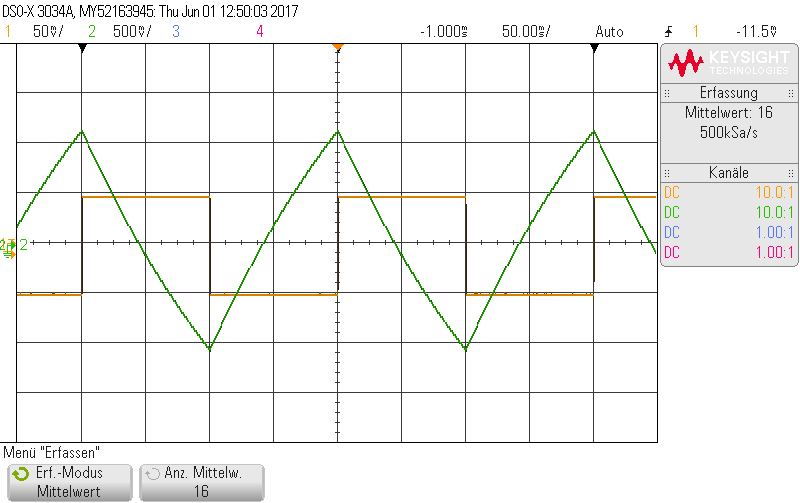
\includegraphics[height=6cm,width=12cm]{OsziBilder/invInte_bigScal.png}
 \end{center}
 \caption{Rechteckspannung $0,1V_{pp}$, $5Hz$ ($U_e$ orange, $U_a$ grün)}
\end{figure}
Jede Halbwelle des Eingangssignales entspricht einem Sprung und dieser integriert ergibt eine Gerade. Da es sich um einen invertierenden Integrierer handelt l\"auft die Gerade immer entegen der Sprungrichtung. In der Abbildung ist genau dieses Verhalten zu erkennen, springt die Eingangspannung ins Negative, entspricht die Ausgnagsspannung einer Geraden mit positiver Steigung, springt die Eingangsspannung ins Positive so ist die Ausgangsspannung eine Gerade mit negativer Steigung.
Die Ausgangsspannung ist, wie man in der Abbildung sehen kann, keine genaue gerade, sondern der Anfang der Lade- bzw. Entladekurve des Kondensators. Wird jedoch über ein kleines Intervall integriert, so entspricht dies annähernd einer Geraden.\\
\newpage
\subsection{Erl\"auterung der Schaltung}
\begin{figure}[H]
  \centering
  \begin{tabular}{ccc}
    & & Ohm'sches Gesetz an $C$ \\
    & & $I=C*\frac{du}{dt}$ \\ \\
    Ohm'sches Gesetz an $R$& & $du = \frac{I*dt}{C}$ \\ \\
    $I=\frac{U_e}{R}$ & & $U_a=\frac{1}{C}\int I dt$ \\
    & Zusammenf\"uhrung der Formeln & \\
    & $U_a = -\frac{1}{C} \int \frac{U_e}{R} dt$ & \\ \\
    & $U_a = -\frac{1}{RC} \int U_e dt$ & \\
  \end{tabular}
  \caption{Formeln zur Berechnung des Integrierers}
\end{figure}
\noindent
Da auf Grund des hohen Eingangswiderstandes kein Strom in den OPV flie\ss{}t, ist auch der Strom durch den Widerstand und Kondensator nahezu ident. Dieser Strom l\"asst sich sowohl am Widerstand als auch am Kondensator durch das Ohm'sche Gesetz berechnen. Formt man nun das Ohm'sche Gesetz von $C$ nach $du$ um, so erh\"alt man eine Differntialgleichung 1. Ordnung. Diese l\"asst sich durch Integrieren l\"osen und es ergibt sich eine Formel zur Berechnung von $U_a$. Setzt man nun die Berechnung f\"ur $I$ am Widerstand in die Umgeformte Formel von $C$ ein erh\"alt man die Formel zur Berechnung der Ausgangsspannung. \\ \\
$U_a = -\frac{1}{RC} \int U_e dt$ \\  \\
Diese Formel besagt, dass die Ausgangsspannung das Integral der Eingangsspannung mit dem Proportionalit\"atsfaktor $\frac{1}{RC}$ ist. \\ \\
Die Integriererschaltung wird häufig in der Regelungstechnik, zB. f\"ur Integralrelger (PI-, PID-Regler), verwendet.

\newpage

% !TEX root = deckblatt3b.tex

\section{Invertierender Schmitt-Trigger}

In dieser Aufgabe war der Operationsverstärker als invertierender Schmitt-Trigger zu beschalten und dessen Funktionsweise zu erproben.\\

\subsection{Schaltung}

\begin{figure}[H]
  \begin{center}
    %\tikzset{component/.style={draw,thick,circle,fill=white,minimum size =0.75cm,inner sep=0pt}}
    \resizebox{0.7\linewidth}{!}{
      \begin{circuitikz}
      \draw (0,0)
      (3,4) node[op amp] (opamp) {}
      (3,4.5) to[short] (3,5) node[vcc] {$V_{CC}$}
      (3,3.5) to[short] (3,3) node[ground](ground) {}
      (opamp.-) to[short] (-2,4.5)
      (opamp.+) to[short] (1.5,3.5) to[short] (1.5,1.5) to[short] (4.5,1.5){}
      (4.5,4) to[R={$R_2$}] (4.5,1.5) to[R={$R_1$}] (4.5,-0.5) node[ground] (ground) {}
      (opamp.out) to[short] (8,4)
      (1.5,1.5) to[R={$R_3$}] (-1, 1.5) to [voltage source, v>=$V_{CC}$] (-1, -0.5) node[ground](ground) {}
      (8,-0.5) node[ground] (ground) {}
      (-2,-0.5) node[ground] (ground) {}
      ;
      \draw (-2,4.2) to[short] (-2,0.2) node[vee] {};
      \draw (-2.5,2.2) node[] {$U_e$};
      \draw (8,3.7) to[short] (8,0.2) node[vee] {};
      \draw (8.5,1.7) node[] {$U_a$};
      \draw (4,1.1) to[short] (4,0.3) node [vee] {};
      \draw (3.5,0.6) node[] {$U_t$};

      \end{circuitikz}
    }  
    \caption{inververtierender Schmitt-Trigger}
  \end{center}
\end{figure}
\noindent

\begin{figure}[H]
 \begin{center}
  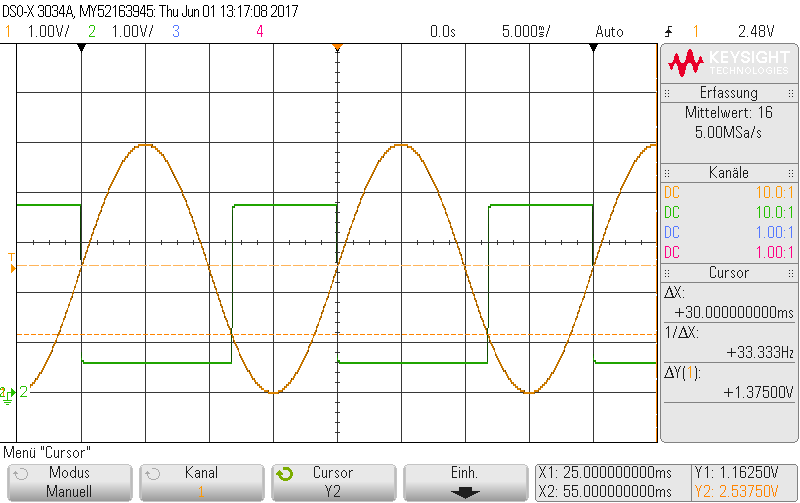
\includegraphics[height=6cm,width=12cm]{OsziBilder/SchmittTrigger_Time}
 \end{center}
 \caption{Zeitverlauf invertierender Schmitt-Trigger, $U_e$ orange und $U_a$ grün}
\end{figure}
\noindent
\newpage
Der Schmitt-Trigger ist eine mitgekoppelte Operationsverstärkerschaltung. Seine Schaltschwellen liegen im allgemeinen symmetrisch
um den Nullpunkt. Durch das Anlegen einer Referenzspannung können die Schaltpunkte für das Über- bzw Untersteuern auch nicht
symmetrisch angesetzt werden. Wird die positive Schaltschwelle erreicht, wird am Ausgang die negative Versorgungsspannung
des OPV's ausgegeben (hier $0V$, Masse). Wird die negative Schaltschwelle erreicht, wird die positive Versorgungsspannung
ausgegeben (hier $V_{CC} = 5V$), diese wird allerdings nicht ganz erreicht, da es sich hier nicht um eine Rail-to-Rail OPV handelt.\\
\\
$U_e=$ Sinus $5V_{pp}$ $50Hz$ Offset $2,5V$, $V_{CC} = +5V$, $R_1=R_2=4,7k\Omega$, $R_3=10k\Omega$\\
gemessen: $U_a=3,18V$, $U_t=1,72V$\\

\subsection{Hysterese}

\begin{figure}[H]
 \begin{center}
  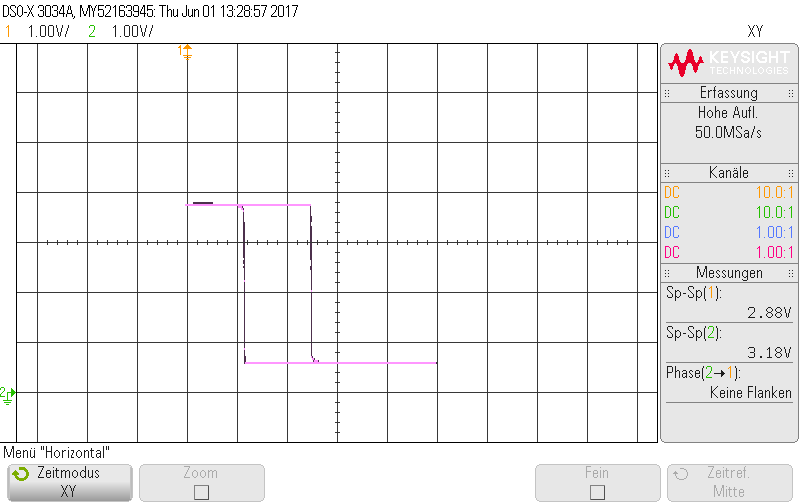
\includegraphics[height=6cm,width=12cm]{OsziBilder/SchmittTrigger_XY}
 \end{center}
 \caption{Hysterese-Kennlinie, x-Achse $U_e$, y-Achse $U_a$}
\end{figure}
\noindent
Die Hysterese-Kennlinie zeigt die Schaltpunkte des Triggers, diese werden durch den von der
Ausgangsspannung beeinflussten Spannungsabfall am Widerstand $R_1$ verschoben. Die aus der Simulation
berechneten Schaltpunkte sind, $U_{low}=0,963V$ und $U_{high}=2,728V$. Diese sind auch mit kleineren
Abweichungen in der Kennlinie zu erkennen, $U_{low}\approx 1,1V$ und $U_{high}\approx 2,25V$.\\
\\
Der Schmitt-Trigger wird zur digitalisierung von Signalen eingesetzt. Eine Hysterese wird hierbei benötigt,
da an den Schaltflanken oft Störsignale ein mehrfaches Über- bzw. Untersteuern des Operationsverstärkers verursachen, was
zu falschen Codierungen führen kann.

% !TEX root = deckblatt3b.tex

\section{Anhang}

\begin{figure}[H]
\centering
\resizebox{0.5\linewidth}{!}{
  \csvautobooktabular{./csv_files/bode1_messdaten.csv}
  }
  \caption{Messwerte f\"ur Figure 11 \& 12}
\end{figure}

\begin{figure}[H]
  \centering
  \resizebox{0.5\linewidth}{!}{
  \csvautobooktabular{./csv_files/bode2_messdaten.csv}
  }
 \caption{Messwerte f\"ur Figure 13 \& 14}
\end{figure}


\end{document}
